\subsection{General structure}

\begin{figure}
	\centering
	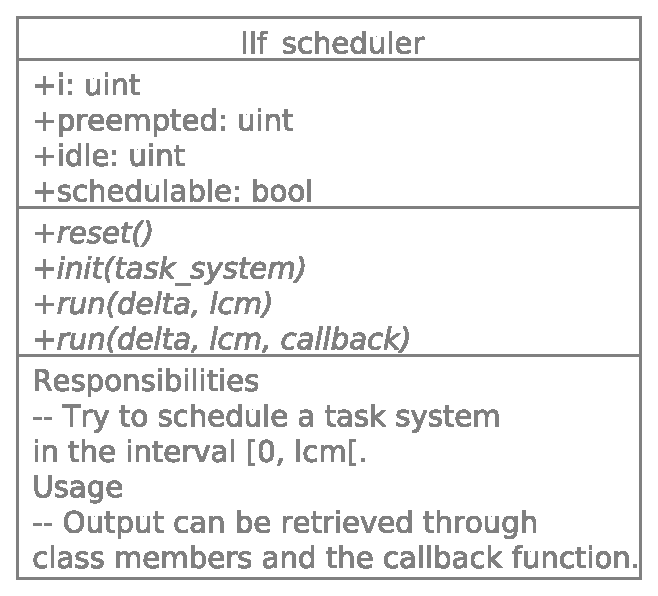
\includegraphics[width=0.5\textwidth]{fig/sim/1}
	\caption{\label{fig:sim:1} Interface of a scheduler}
\end{figure}

 \ref{fig:sim:1} describes the interface of both implementations. A use case can be seen in \ref{code:sim:1}.

\myinputminted[firstline=154,lastline=157]{c++}{../src/simLLF.cpp}{Use case of the scheduler interface}{code:sim:1}{3}

\nb{All the functionalities are splitted into small tools with aim to better flexibility, so for example in \ref{code:sim:1} you can see that the \emph{lowest common multiple} is computed outside of the scheduler.}